\chapter{Ergebnisse}

Sämtlichen Ergebisse wurden im BwUniCluster2.0 erzeugt. Sofern nicht anders erwähnt wurden
2x Intel Xeon Gold 6230
180GB RAM verwendet.

Die bereitgestellten Graphen mussten vor ihrer Nutzung gereinigt und an die Implementierung angepasst werden.
Sie enthielten isolierte Knoten, und die Kantengewichte der Sichtbarkeitsgraphen waren als Gleitkommazahlen gespeichert.
Für die Anpassung wurde ein Python-Skript benutzt, das folgende Aufgaben durchführt:

\begin{itemize}
    \item
          Transformation der Kantengewichte.

    \item
          Entfernung isolierter Knoten.

    \item
          Anpassung der Knoten-IDs, sodass die Knoten-IDs im Sichtbarkeitsgraphen den Bereich $0, \dotsc, n$ und im triangulierten Graphen den Bereich $0, \dotsc, n + m$ umfassen.
\end{itemize}

Während der Untersuchung der triangulierten Graphen wurde festgestellt, dass einige Kanten ein Gewicht von 0 aufwiesen.
Diese Kanten wurden unverändert beibehalten.

medi und pata Sichtbarkeitsgraphen fehlten jeweils einige Kanten, damit sie ungerichtet sind.
Diese wurden von Hand ergänzt.

\section{Untersuchung der Graphen}

Die Sichtbarkeitsgraphen wurden auf die Verteilung der Kantengrade untersucht.
Dabei wurden die folgenden Histogramme erstellt.
Für jeden der Sichtbarkeitsgraphen gilt, dass mindestens 90\% aller Knoten einen Grad kleiner \num{2000} haben.

\begin{figure}[!ht]
    \begin{subfigure}[b]{0.5\textwidth}
        \resizebox{\textwidth}{!}{%
            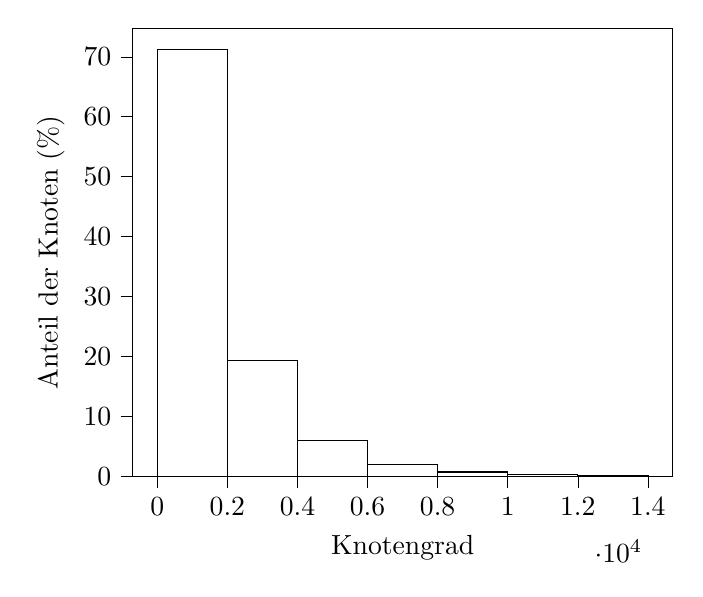
\begin{tikzpicture}
                \begin{axis}[
                        tick align=outside,
                        tick pos=left,
                        xmin=-698, xmax=14702,
                        xtick style={color=black},
                        xtick distance=2000,
                        ymin=0, ymax=0.747618384401001,
                        ytick style={color=black},
                        ytick={0,0.1,0.2,0.3,0.4,0.5,0.6,0.7,0.8},
                        yticklabels={0,10,20,30,40,50,60,70,80},
                        xlabel={Knotengrad},
                        ylabel={Anteil der Knoten (\%)}
                    ]
                    \draw[] (axis cs:2,0) rectangle (axis cs:2002,0.712017508953334);
                    \draw[] (axis cs:2002,0) rectangle (axis cs:4002,0.194220055711032);
                    \draw[] (axis cs:4002,0) rectangle (axis cs:6002,0.0606247512935969);
                    \draw[] (axis cs:6002,0) rectangle (axis cs:8002,0.0205382013530728);
                    \draw[] (axis cs:8002,0) rectangle (axis cs:10002,0.00766514126545947);
                    \draw[] (axis cs:10002,0) rectangle (axis cs:12002,0.00397930760049903);
                    \draw[] (axis cs:12002,0) rectangle (axis cs:14002,0.000955033824119655);
                \end{axis}
            \end{tikzpicture}
        }
        \caption{aegaeis-vis}
    \end{subfigure}%
    \begin{subfigure}[b]{0.5\textwidth}
        \resizebox{\textwidth}{!}{%
            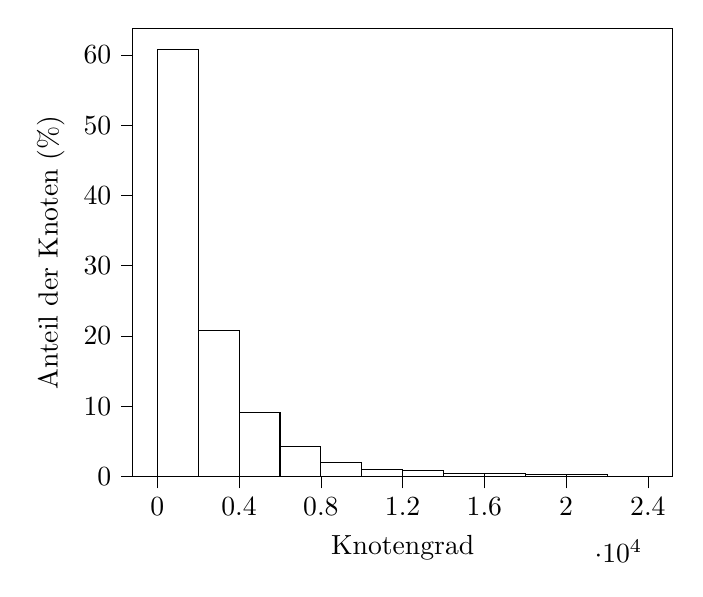
\begin{tikzpicture}
                \begin{axis}[
                        tick align=outside,
                        tick pos=left,
                        xlabel={Knotengrad},
                        xmin=-1198, xmax=25202,
                        xtick distance=4000,
                        xtick style={color=black},
                        ylabel={Anteil der Knoten (\%)},
                        ymin=0, ymax=0.637890337808629,
                        ytick style={color=black},
                        ytick={0,0.1,0.2,0.3,0.4,0.5,0.6,0.7},
                        yticklabels={0,10,20,30,40,50,60,70}
                    ]
                    \draw[] (axis cs:2,0) rectangle (axis cs:2002,0.60751460743679);
                    \draw[] (axis cs:2002,0) rectangle (axis cs:4002,0.207212784893063);
                    \draw[] (axis cs:4002,0) rectangle (axis cs:6002,0.0905080679486225);
                    \draw[] (axis cs:6002,0) rectangle (axis cs:8002,0.0423164235317719);
                    \draw[] (axis cs:8002,0) rectangle (axis cs:10002,0.0196700589456533);
                    \draw[] (axis cs:10002,0) rectangle (axis cs:12002,0.0103219440467273);
                    \draw[] (axis cs:12002,0) rectangle (axis cs:14002,0.00818403436132265);
                    \draw[] (axis cs:14002,0) rectangle (axis cs:16002,0.00425647177184629);
                    \draw[] (axis cs:16002,0) rectangle (axis cs:18002,0.00420165357478464);
                    \draw[] (axis cs:18002,0) rectangle (axis cs:20002,0.00342452501643997);
                    \draw[] (axis cs:20002,0) rectangle (axis cs:22002,0.00236363167330556);
                    \draw[] (axis cs:22002,0) rectangle (axis cs:24002,2.57967986172503e-05);
                \end{axis}
            \end{tikzpicture}
        }
        \caption{medi-vis}
    \end{subfigure}
    \par\bigskip
    \begin{subfigure}[b]{0.5\textwidth}
        \resizebox{\textwidth}{!}{%
            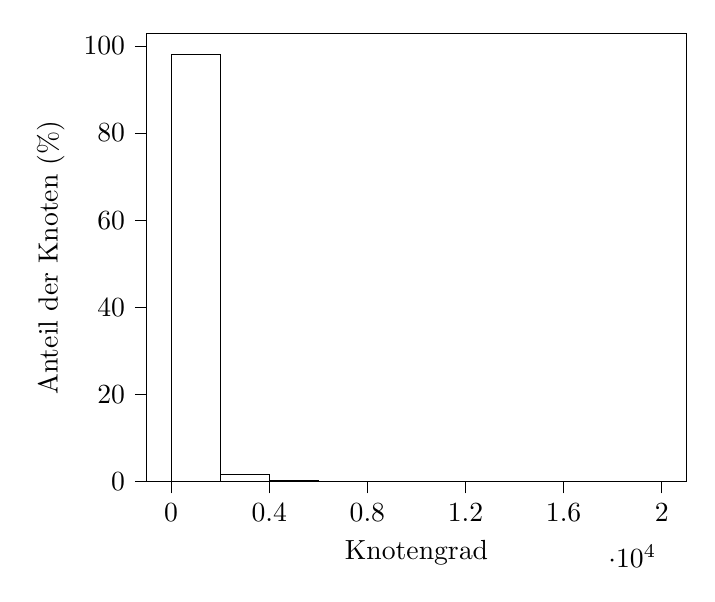
\begin{tikzpicture}
                \begin{axis}[
                        tick align=outside,
                        tick pos=left,
                        xlabel={Knotengrad},
                        ylabel={Anteil der Knoten (\%)},
                        xmin=-998, xmax=21002,
                        xtick style={color=black},
                        y grid style={darkgray176},
                        xtick distance=4000,
                        ymin=0, ymax=1.02857224104146,
                        ytick style={color=black},
                        ytick={0,0.2,0.4,0.6,0.8,1,1.2},
                        yticklabels={0,20,40,60,80,100,120}
                    ]
                    \draw[] (axis cs:2,0) rectangle (axis cs:2002,0.979592610515676);
                    \draw[] (axis cs:2002,0) rectangle (axis cs:4002,0.0169022235303201);
                    \draw[] (axis cs:4002,0) rectangle (axis cs:6002,0.00222602483448042);
                    \draw[] (axis cs:6002,0) rectangle (axis cs:8002,0.000968834654540784);
                    \draw[] (axis cs:8002,0) rectangle (axis cs:10002,0.000297335455255565);
                    \draw[] (axis cs:10002,0) rectangle (axis cs:12002,3.99107993631631e-06);
                    \draw[] (axis cs:12002,0) rectangle (axis cs:14002,0);
                    \draw[] (axis cs:14002,0) rectangle (axis cs:16002,9.97769984079078e-07);
                    \draw[] (axis cs:16002,0) rectangle (axis cs:18002,3.99107993642733e-06);
                    \draw[] (axis cs:18002,0) rectangle (axis cs:20002,3.99107993631631e-06);
                \end{axis}

            \end{tikzpicture}
        }
        \caption{pata-vis}
    \end{subfigure}
    \caption{Verteilung der Kantengrade}
\end{figure}

Für die Laufzeit der Kontraktion die Summe der quadratischen Knotengrade bedeutsam.
Diese sind in \autoref{table:sum_quad_degree} sichtbar.
Obwohl pata die meisten Knoten hat, ist die summe der Quadrate am kleinsten.
Vielleicht geht ch witness doch?

\begin{table}[ht]
    \centering
    \begin{tabular}{
            l % Graph
            S[table-format = 13.0] % Zeit
        }
        \toprule
        {Graph}            & {$\sum_{v \in V} (\text{Grad}(v))^2$} \\ \midrule
        aegaeis-visibility & 1153579966074                         \\
        medi-visibility    & 4667069733248                         \\
        pata-visibility    & 426189267238                          \\ \bottomrule
    \end{tabular}
    \caption{Summe quadratische Knotengrade}
    \label{table:sum_quad_degree}
\end{table}

\begin{figure}[!ht]% Die Daten in den .csv Dateien sind gelippt auf 100. pgf hat Probleme mit zu großen Zahlen.
    \begin{subfigure}[b]{0.5\textwidth}
        \resizebox{\textwidth}{!}{%
            \begin{tikzpicture}
                \begin{axis}[
                        ymax=6,
                        xlabel={Hop-Länge},
                        ylabel={Fehler (\%)},
                        legend style={at={(1,0.475)},anchor=east, nodes={scale=0.8, transform shape}}
                    ]
                    \addplot+[mark repeat=7] table [x=hops, y=simple_graph_upper_bound, col sep=comma] {data/bounds/aegaeis.csv};
                    \addlegendentry{$\triangle$};

                    \addplot+[mark repeat=7] table [x=hops, y=10, col sep=comma] {data/bounds/aegaeis.csv};
                    \addlegendentry{10 Hubs};

                    \addplot+[mark repeat=7] table [x=hops, y=20, col sep=comma] {data/bounds/aegaeis.csv};
                    \addlegendentry{20 Hubs};

                    \addplot+[mark repeat=7] table [x=hops, y=40, col sep=comma] {data/bounds/aegaeis.csv};
                    \addlegendentry{40 Hubs};

                    \addplot+[mark repeat=7] table [x=hops, y=80, col sep=comma] {data/bounds/aegaeis.csv};
                    \addlegendentry{80 Hubs};

                    \addplot+[mark repeat=7] table [x=hops, y=min_80_simple, col sep=comma] {data/bounds/aegaeis.csv};
                    \addlegendentry{$\triangle$, 80 Hubs};
                \end{axis}
            \end{tikzpicture}
        }
        \caption{aegaeis-vis}
    \end{subfigure}%
    \begin{subfigure}[b]{0.5\textwidth}
        \resizebox{\textwidth}{!}{%
            \begin{tikzpicture}
                \begin{axis}[
                        ymax=6,
                        xlabel={Hop-Länge},
                        ylabel={Fehler (\%)},
                        legend style={at={(1,0.475)},anchor=east, nodes={scale=0.8, transform shape}}
                    ]
                    \addplot+[mark repeat=7] table [x=hops, y=simple_graph_upper_bound, col sep=comma] {data/bounds/medi.csv};
                    \addlegendentry{$\triangle$};

                    \addplot+[mark repeat=7] table [x=hops, y=10, col sep=comma] {data/bounds/medi.csv};
                    \addlegendentry{10 Hubs};

                    \addplot+[mark repeat=7] table [x=hops, y=20, col sep=comma] {data/bounds/medi.csv};
                    \addlegendentry{20 Hubs};

                    \addplot+[mark repeat=7] table [x=hops, y=40, col sep=comma] {data/bounds/medi.csv};
                    \addlegendentry{40 Hubs};

                    \addplot+[mark repeat=7] table [x=hops, y=80, col sep=comma] {data/bounds/medi.csv};
                    \addlegendentry{80 Hubs};

                    \addplot+[mark repeat=7] table [x=hops, y=min_80_simple, col sep=comma] {data/bounds/medi.csv};
                    \addlegendentry{$\triangle$, 80 Hubs};
                \end{axis}
            \end{tikzpicture}
        }
        \caption{medi-vis}
    \end{subfigure}
    \par\bigskip
    \begin{subfigure}[b]{0.5\textwidth}
        \resizebox{\textwidth}{!}{%
            \begin{tikzpicture}
                \begin{axis}[
                        ymax=6,
                        xlabel={Hop-Länge},
                        ylabel={Fehler (\%)},
                        legend style={at={(1,0.475)},anchor=east, nodes={scale=0.8, transform shape}}
                    ]
                    \addplot+[mark repeat=7] table [x=hops, y=simple_graph_upper_bound, col sep=comma] {data/bounds/pata.csv};
                    \addlegendentry{$\triangle$};

                    \addplot+[mark repeat=7] table [x=hops, y=10, col sep=comma] {data/bounds/pata.csv};
                    \addlegendentry{10 Hubs};

                    \addplot+[mark repeat=7] table [x=hops, y=20, col sep=comma] {data/bounds/pata.csv};
                    \addlegendentry{20 Hubs};

                    \addplot+[mark repeat=7] table [x=hops, y=40, col sep=comma] {data/bounds/pata.csv};
                    \addlegendentry{40 Hubs};

                    \addplot+[mark repeat=7] table [x=hops, y=80, col sep=comma] {data/bounds/pata.csv};
                    \addlegendentry{80 Hubs};

                    \addplot+[mark repeat=7] table [x=hops, y=min_80_simple, col sep=comma] {data/bounds/pata.csv};
                    \addlegendentry{$\triangle$, 80 Hubs};
                \end{axis}
            \end{tikzpicture}
        }
        \caption{pata}
    \end{subfigure}
    \caption{Fehler der oberen Schranken}
\end{figure}

aegaeis
75.6658\% korrekt
0.40990444596118253 average

%WARUM MEDI, PATA nicht so korrekt?
\todo{STIMMEN ZAHLEN?}

medi
0.39110000000000006\% korrekt
0.9727677753480117 average

pata
0.068\% korrekt
0.6179520250326755 average




vergleich der Abstände im vis und graph, sortiert nach hops in vis.

Heuristic egde difference (zufall)
Vis graphen haben sehr hohen degree (TODO Beweis).
Daher degree x degree viele checks, das gehtn schnell in die Millionen bis Milliarden.
Idee: betrachte nur ein Subset (tails, heads) und schaue ob und wie genau dieses die Edge difference aproximiert.

Das kann dann wieder für andere Methoden benutzt werden.

Plot hitting set vs bottom-up order

\section{Dijkstra}

Für die Berechnung des Speedups der in dieser Arbeit angewandeten Methoden wurden für jeden Graph \num{1000} sequentielle $s-t$ Dijkstra-Suchen asugeführt und die durschnittliche Laufzeit ermittelt.
Die durschnittliche Laufzeiten für das Finden und erstellen des kürzesten Pfad sind in Tabelle \ref{ergebnisse::table:dijkstra_one_to_one} dargestellt.
Es ist ersichtlich, dass die Sichtbarkeitsgraphen im Vergleich zu ihren Triangulierungen deutlich höhere Laufzeiten haben.

\begin{table}[ht]
    \centering
    \begin{tabular}{
            l % Graph
            S[table-format = 4.1] % Zeit
        }
        \toprule
        {Graph}            & {$\varnothing$ $t({spd})$} \\
        {}                 & {ms}                       \\ \midrule
        aegaeis-graph      & 60.281198                  \\
        aegaeis-visibility & 630.434928                 \\
        medi-graph         & 87.08376                   \\
        medi-visibility    & 1279.67479                 \\
        pata-graph         & 265.825771                 \\
        pata-visibility    & 1017.695977                \\ \bottomrule
    \end{tabular}
    \caption{Durchschnitliche Laufzeit einer Dijkstra Suche}
    \label{ergebnisse::table:dijkstra_one_to_one}
\end{table}

Zusätzlich zur durschnitlichen Laufzeit wurde die die Durschnitswerte der Hop-Länge, des Dijsktra-Rank und der Queue pops ermittelt, um ein Verständnis für die Laufzeiten zu erlangen.
Es zeigte sich, dass die durschnittliche Hop-Länge der Sichtbarkeitsgraphen deutlich signifikant kürzer ist, als die der Triangulierungen.
Obwohl die Sichtbarkeitsgraphen eine niedriger Anzahl an Knoten haben, ist die durschnitliche Anzahl der Queue pops größer.
Dies legt Nahe, dass die verwendung einer Warteschlange, welche eine \emph{Drecrease-Key} Funktion anbietet, die Geschwindigkeit der Dijkstra Suche erhöhen würde.

\begin{table}[ht]
    \centering
    \begin{tabular}{
            l % Graph
            S[table-format = 3.1] % hop-länge
            S[table-format = 7.0] % rank
            S[table-format = 7.0] % queue pops
        }
        \toprule
        {Graph}            & {$\varnothing$  Hop-Länge} & {$\varnothing$ Dijkstra Rank} & {$\varnothing$ Queue pops} \\ \midrule
        aegaeis-graph      & 215.7201                   & 260447.36                     & 325845.56                  \\
        aegaeis-visibility & 16.311                     & 98650.82                      & 517346.63                  \\
        medi-graph         & 340.445                    & 394855.78                     & 494553.97                  \\
        medi-visibility    & 23.6149                    & 154092.42                     & 959206.4                   \\
        pata-graph         & 883.979                    & 1120841.9                     & 1387047.8                  \\
        pata-visibility    & 63.817                     & 498570.2                      & 2429689.8                  \\ \bottomrule
    \end{tabular}
    \caption{Durschnitliche Kennwerte der Dijkstra Suchen (über \num{10000} Suchen)}
\end{table}

\section{CH mit Witness}

Es wurde versucht die CH mit Witness, Edge Difference, Lacy Popping zu erstellen.
Dies hat für die Sichtbarkeitsgraphen nicht funktioniert, da 3 Tage nicht ausreichten die Graphen zu erzeugen.
Die Suche ist einfach zu teuer.
Pro Vorgänger muss eine Suche zu allen Nachfolgern gemacht werden.

\begin{table}[ht]
    \centering
    \begin{tabular}{
            l % Graph
            S[table-format = 1.2] % creation zeit
            S[table-format = 4.1] % average time
            S[table-format = 4.1] % speedup
        }
        \toprule
        {Graph}       & {Erstellung}  & {$\varnothing$ $t({spd})$} & {speedup} \\
        {}            & {(min)}       & {(µs)}                     & {}        \\ \midrule
        aegaeis-graph & 2.1336        & 514.069                    & 117.263   \\
        medi-graph    & 3.08033333333 & 543.803                    & 160.138   \\
        pata-graph    & 9.84055       & 730.317                    & 363.987   \\\bottomrule
    \end{tabular}
    \caption{ch one-to-one, averaged over 1000 sequential searches}
\end{table}

\section{CH All-In}

All in sortiert nach all in edge differnce:

\section{Hitting Set}

Für die Graphen wurden jeweils ein Hitting Set über \num{100000} Pfade erstellt.
Diese Pfade wurden mit Dijkstra erstellt.
Die dafür benötigte Zeit ist in der \autoref{table:ergebnisse:100k_hitting_set_time} angeben.
Es hätte durchaus mehr Zeit in mehr Pfade gesteckt werden können, jedoch wurde bewusste wenig Aufwand darin gesteckt.
Wenn das auch auch so funktioniert, dann kann mit den Speedup Techniken viel schneller viel mehr PFade generiert werden.

\begin{table}[ht]
    \centering
    \begin{tabular}{
            l % Graph
            S[table-format = 4.0] % creation zeit
        }
        \toprule
        {Graph}            & {Erstellung}       \\
        {}                 & {(min)}            \\ \midrule
        aegaeis-graph      & 3.4333333333333336 \\
        aegaeis-visibility & 47.65              \\
        medi-graph         & 4.883333333333333  \\
        medi-visibility    & 102.38333333333334 \\
        pata-graph         & 12.35              \\
        pata-visibility    & 62.81666666666667  \\  \bottomrule
    \end{tabular}
    \caption{Erstellung eines Hitting-Set über \num{100000} Pfade, welche mit Dijkstra-Suchen erzeugt wurden}
    \label{table:ergebnisse:100k_hitting_set_time}
\end{table}

Wie hitbar sind die Graphen? plote hit percentage

\section{PEOPLE}

Die in \autoref{chapter:peopel} vorgestellte Methode zur Berechnung von Contracted und Hub Graphen lies sie auch die Sichtbarkeitsgraphen und ihre Triangulierungen anwenden.

\subsection{Contracted Graph}

Die in \autoref{chapter:peopel} vorgestellte Methode zur Berechnung eines Contracted Graphens lies sich auf alle Graphen anwenden.
Die erzielten Werte der ERstellung sind in \autoref{table:ergebnisse:people_ch_erstellung} gesammelt.
Anzahl der Abkürzungen in Relation zu Anzahl der ursprünglichen Kanten.

\begin{table}[ht]
    \centering
    \begin{tabular}{
            l % Graph
            S[table-format = 4.0] % creation zeit
            S[table-format = 9.0] % shortcuts added
            S[table-format = 4.1] % Knotengrad
        }
        \toprule
        {Graph}            & {Erstellung}       & {Abkürzungen} & {$\varnothing$ Grad} \\
        {}                 & {(min)}            & {}            & {}                   \\ \midrule
        aegaeis-graph      & 20.2               & 12443056      & 14.515443            \\
        aegaeis-visibility & 353.81666666666666 & 214987558     & 1288.5282            \\
        medi-graph         & 38.21666666666667  & 20003908      & 15.2253065           \\
        medi-visibility    & 1252.6666666666667 & 468641256     & 1913.623             \\
        pata-graph         & 342.1666666666667  & 70624466      & 18.35748             \\
        pata-visibility    & 2685.0833333333335 & 613324174     & 457.05353            \\  \bottomrule
    \end{tabular}
    \caption{Erstellung von Contracted Graphen mit PEOPLE}
    \label{table:ergebnisse:people_ch_erstellung}
\end{table}

Der Speedup ist in \autoref{table:ergebnisse:people_ch_speedup} zusammgenfasst.
Der Speedup der Trianuglierten Graphen ist deutlich kleiner, als der mit CH Witness, jedoch eine größenordnung schneller.
Der Speedup der Sichtbarkeitsgraphen ist kleines als eine Größenordnung.
Das sollte noch erkundet werden, warum.

pata hat trotzem mehr Speedup, weil von der Struktur her schon fast ein Straßengraph

\begin{table}[ht]
    \centering
    \begin{tabular}{
            l % Graph
            S[table-format = 3.2] % average time spd
            S[table-format = 3.2] % speedup
        }
        \toprule
        {Graph}            & {$\varnothing$ $t({spd})$} & {Speedup}          \\
        {}                 & {(ms)}                     & {}                 \\ \midrule
        aegaeis-graph      & 2.337158                   & 25.792521515447394 \\
        aegaeis-visibility & 443.650843                 & 1.421015958714182  \\
        medi-graph         & 3.443191                   & 25.291585625078596 \\
        medi-visibility    & 938.863249                 & 1.363004453910625  \\
        pata-graph         & 10.199549                  & 26.062502469471934 \\
        pata-visibility    & 257.635631                 & 3.950136761168722  \\  \bottomrule
    \end{tabular}
    \caption{Speedup der mit PEOPLE erstellten Contracted Graphen}
    \label{table:ergebnisse:people_ch_speedup}
\end{table}

\subsection{Hub Graph}

\subsubsection{Bootstraping HL}

Das Merging war deutlicht teruer als erwartet.
Dies ist dadurch zu erklären, dass für jeden Knoten die Anzahl der ausgehenden Contrated Graph Knoten viele Labels gemerged werden, welche durschnitlich sehr groß sind.
Das Mergen lässt sich aber gut parallisieren, durch eine Fold Operation, bei der jeder Thread für sich eine Menge an Labels merged.

\begin{table}[ht]
    \centering
    \begin{tabular}{ % DIREKT
            l % Graph
            S[table-format = 4.0] % creation zeit
            S[table-format = 4.1] % average time
        }
        \toprule
        {Graph}            & {Erstellung}       & {$\varnothing$ Label Größe} \\
        {}                 & {(min)}            & {}                          \\ \midrule
        aegaeis-graph      & 86.55              & 225.21998319619112          \\
        aegaeis-visibility & 357.9166666666667  & 2447.866444488659           \\
        medi-graph         & 191.06666666666666 & 262.34248736183486          \\
        medi-visibility    & 1317.85            & 3528.6126965393596          \\
        pata-graph         & 1706.5333333333333 & 451.8001829187458           \\
        pata-visibility    & 2657.5             & 1823.062327697596           \\  \bottomrule
    \end{tabular}
    \caption{Erstellung von Hub Graphen mit PEOPLE}
\end{table}

\subsubsection{Direkt HL}

Das Anwenden des des Algorithmus zur Berechnung des Hub GRaphens hat gut funktioniert.
\todo{DIE LABELS SIND MINIMAL UNTERSCHIEDLICH GROß}

\begin{table}[ht]
    \centering
    \begin{tabular}{% MERGE ONLY
            l % Graph
            S[table-format = 4.0] % creation zeit
            S[table-format = 4.1] % average time
        }
        \toprule
        {Graph}            & {Erstellung}       & {$\varnothing$ Label Größe} \\
        {}                 & {(min)}            & {}                          \\ \midrule
        aegaeis-graph      & 12.3               & 225.18963155458096          \\
        aegaeis-visibility & 455.48333333333335 & 2446.9511241543973          \\
        medi-graph         & 19.75              & 262.32183266591755          \\
        medi-visibility    & 1338.4833333333333 & 3527.5645951837378          \\
        pata-graph         & 82.48333333333333  & 451.71017734369667          \\
        pata-visibility    & 847.2833333333333  & 1822.0561604813242          \\  \bottomrule
    \end{tabular}
    \caption{Erstellung von Hub Graphen durch Merging der mit PEOPLE erzeugen Contracted Graphen}
\end{table}

\subsubsection{Vergleich}

Für die Sichtbarkeitsgraphen ist es effizienter direkt die HL zu berechen.
Für die Triangulierten gRaphen ist es effizietner zuerst die  Contrated Graphen zu berechen.


\begin{table}[ht]
    \centering
    \begin{tabular}{ %VERGLEICH
            l % Graph
            S[table-format = 4.0] % creation zeit
            S[table-format = 4.0] % average time
        }
        \toprule
        {Graph}            & {CH \& Merging}               & {HL DIREKT}                  \\
        {}                 & {(min)}                       & {(min)}                      \\ \midrule
        aegaeis-graph      & \bfseries 32.5                & 86.55                        \\
        aegaeis-visibility & 809.3                         & \bfseries  357.9166666666667 \\
        medi-graph         & \bfseries  57.96666666666667  & 191.06666666666666           \\
        medi-visibility    & 2591.15                       & \bfseries  1317.85           \\
        pata-graph         & \bfseries  424.65000000000003 & 1706.5333333333333           \\
        pata-visibility    & 3532.366666666667             & \bfseries 2657.5             \\  \bottomrule
    \end{tabular}
    \caption{HL  merged}
\end{table}

\subsubsection{Neuberechnen mit größeren Hitting Set}

Die benutzten Hub Graphen wurden benutzt, um ein großes Hitting Set zu erzeugen.
Es wurde überschlagen, wieviele Pfade 1TB an Speicher ergeben.

\begin{table}[ht]
    \centering
    \begin{tabular}{
            l % Graph
            S[table-format = 4.0] % rank
            S[table-format = 11.0] % queue pops
        }
        \toprule
        {Graph}            & {Speicherbedarf Pfad} & {Pfade}     \\
        {}                 & {Byte}                & {}          \\ \midrule
        aegaeis-graph      & 880                   & 1136363636  \\
        aegaeis-visibility & 84                    & 11904761904 \\
        medi-graph         & 1380                  & 724637681   \\
        medi-visibility    & 112                   & 8928571428  \\
        pata-graph         & 3552                  & 281531531   \\
        pata-visibility    & 272                   & 3676470588  \\ \bottomrule
    \end{tabular}
    \caption{Durschnitliche Kennwerte der Dijkstra Suchen (über \num{10000} Suchen)}
\end{table}

\subsection{Vertex-to-level Vergeleich}

\begin{table}[ht]
    \centering
    \begin{tabular}{
            l % Graph
            S[table-format = 6.0] % random
            S[table-format = 6.0] % degree large to small
            S[table-format = 6.0] % queue pops
        }
        \toprule
        {Graph}            & {random} & {degree (small to large)} & {degree (large to small)} \\ \midrule
        aegaeis-graph      & 3674.8   & 1313.9                    & 22471.6                   \\
        aegaeis-visibility & 17143.0  & 7533.1                    & 57248.0                   \\
        medi-graph         & 3804.2   & 1577.5                    & 32058.1                   \\
        medi-visibility    & 24135.1  & 12791.3                   & 76832.9                   \\
        pata-graph         & 4708.9   & 1639.1                    & 61296.9                   \\
        pata-visibility    & 23282.4  & 10094.1                   & 112915.8                  \\ \bottomrule
    \end{tabular}
    \caption{Predicted HL Label Size, 1000}
\end{table}

\begin{table}[ht]
    \centering
    \begin{tabular}{
            l % Graph
            S[table-format = 6.0] % random
            S[table-format = 6.0] % degree large to small
            S[table-format = 6.0] % queue pops
        }
        \toprule
        {Graph}            & {random} & {degree (small to large)} & {degree (large to small)} \\ \midrule
        aegaeis-graph      & 52.5     & 11.2                      & 941.6                     \\
        aegaeis-visibility & 3110.7   & 905.0                     & 13061.7                   \\
        medi-graph         & 46.8     & 15.0                      & 1299.2                    \\
        medi-visibility    & 4203.9   & 1322.7                    & 16855.0                   \\
        pata-graph         & 31.4     & 9.7                       & 1064.8                    \\
        pata-visibility    & 1305.7   & 264.3                     & 9341.4                    \\ \bottomrule
    \end{tabular}
    \caption{Predicted CH Degree, 1000}
\end{table}
